\documentclass[i1]{oss}
\setlength{\topmargin}{-.5in}
\setlength{\textheight}{9in}
\setlength{\oddsidemargin}{.100in}
\setlength{\textwidth}{6.25in}
\usepackage [dutch] {babel}
\usepackage{graphicx}
\usepackage{amsmath}
\usepackage{fullpage}
\usepackage{color}
\usepackage{soul}
\usepackage{gensymb}
\usepackage{caption}
\usepackage{subcaption}

\begin{document}

\team{6} % teamkleur
\members{Joren Verspeurt {\small \texttt{(r0258417)} } \\
         Sophie Marien {\small \texttt{(s0216517)}}\\
         Stef Noten {\small \texttt{(s0211264)}}\\
         Toon Nolten {\small \texttt{(r0258654)}} } % teamleden

\maketitlepage
\newpage
\tableofcontents
\pagebreak

\section*{Inleiding}

% Een inleiding: beschrijf hierin jullie algemene impressie van het systeem, de manier waarop
% jullie de analyse hebben aangepakt, etc.

%TODO Het Package, testen, klassen
In dit project wordt JUnit geanalyseerd met behulp van visualisatie tools. JUnit is een testing en regression testing framework in Java.\\


Om een eerste inzicht te krijgen in JUnit werd de javadoc geraadpleegd. Door het gericht doorzoeken van deze Javadoc kon een beter zicht op de structuur van JUnit verkregen worden. Hieruit werd dan afgeleid dat er in de source van JUnit twee bijna volledig onafhankelijke versies zitten. Het package junit is een oudere versie (3.8) die in het project zit voor backwards compatibility. Het package org.junit bevat de eigenlijke code van de te analyseren versie. Bij het analyseren van het ontwerp van JUnit werd enkel gekeken naar de huidige versie (exclusief de testen). De testen werden afzonderlijk behandeld.\\

De eerste tool die gebruikt werd om JUnit te analyseren was \emph{CodeCity}. Hiermee kon al direct worden vastgesteld dat JUnit bestaat uit veel klassen die erg klein zijn (drie methodes of minder). Verder werd ook vastgesteld dat er ook relatief veel kleine packages zijn. Er zijn geen duidelijke problemen vast te stellen bij \emph{CodeCity}. De tool vindt in JUnit geen anti-patterns, zoals o.a. God, Brain of Data classes. \\

Voor de verdere analyse werden er andere tools gebruikt en werd er ook manueel door de code genavigeerd om beter inzicht te verwerven. \\

De eerste impressie die we van JUnit kregen is dat er gemiddeld een lage coupling aanwezig is. De functionaliteit is verdeeld over veel klassen waarvan een groot aantal slechts een kleine taak hebben. Een aantal verantwoordelijkheden zijn daarom moeilijk toe te wijzen aan een specifieke klasse omdat ze door samenwerking van verschillende klassen gerealiseerd worden.\\

\section{Ontwerpdocumentatie}

De JUnit-code bestaat uit twee afzonderlijke delen. Het package \emph{junit} behoort tot versie v3.x, dit is aanwezig omwille van backwards compatibility, zodat testsuites voor JUnit v3.x nog gedraaid kunnen worden. Het package \emph{org.junit} bevat de huidige versie (v4.11). Deze twee pakketten zijn bijna volledig onafhankelijk, op een paar klassen na die toelaten om v3.x testen te draaien onder de nieuwere v4.11 architectuur.

Naast het oudere package \emph{junit} zijn er in het huidige package \emph{org.junit} ook een groot aantal klassen gedeclareerd als deprecated, zodat ook dezen eigenlijk niet meer tot het huidige design behoren. De code bevat ook het package \emph{org.junit.experimental}, dat klassen bevat voor features die nog niet stabiel genoeg zijn om tot de offici\"ele release te behoren.

De kern van JUnit is de \emph{org.junit.Runner} klasse. Deze is verantwoordelijk voor het draaien van een of meerdere testen. Binnen JUnit zijn er verschillende implementaties van deze klasse voorzien. 

\subsection{Uitvoering van testen: Runners}

De \emph{org.junit.Runner} klasse is de kern van JUnit. In deze abstracte klasse is een interface vastgelegd voor alle klassen die tests willen draaien. De methode \emph{run(RunNotifier)} op deze klasse dient aangeroepen te worden om de test(en) te draaien die de runner voorstelt. De meegegeven \emph{RunNotifier} wordt door de emph{Runner} aangeroepen bij events in de testflow. Ge\"interesseerde objecten kunnen zich inschrijven bij deze \emph{RunNotifier} om op de hoogte gehouden te worden van de voortgang van de testrun (Observable patroon).

Er zijn verschillende implementaties aanwezig van de \emph{Runner} klasse, in figuur \ref{fig:diagrams:Runner} is een selectie te zien. De interessantste is de \emph{org.junit.runners.ParentRunner}. Deze klasse maakt het mogelijk om een hi\"erarchie te maken voor het runnen van testen: hij bevat children die zelf opnieuw gerunned kunnen worden. Hij laat ook toe om zijn childtesten te sorteren en filteren (met aparte \emph{Filter} en \emph{Sorter} klassen).

\begin{figure}[hb!]
	\centering
	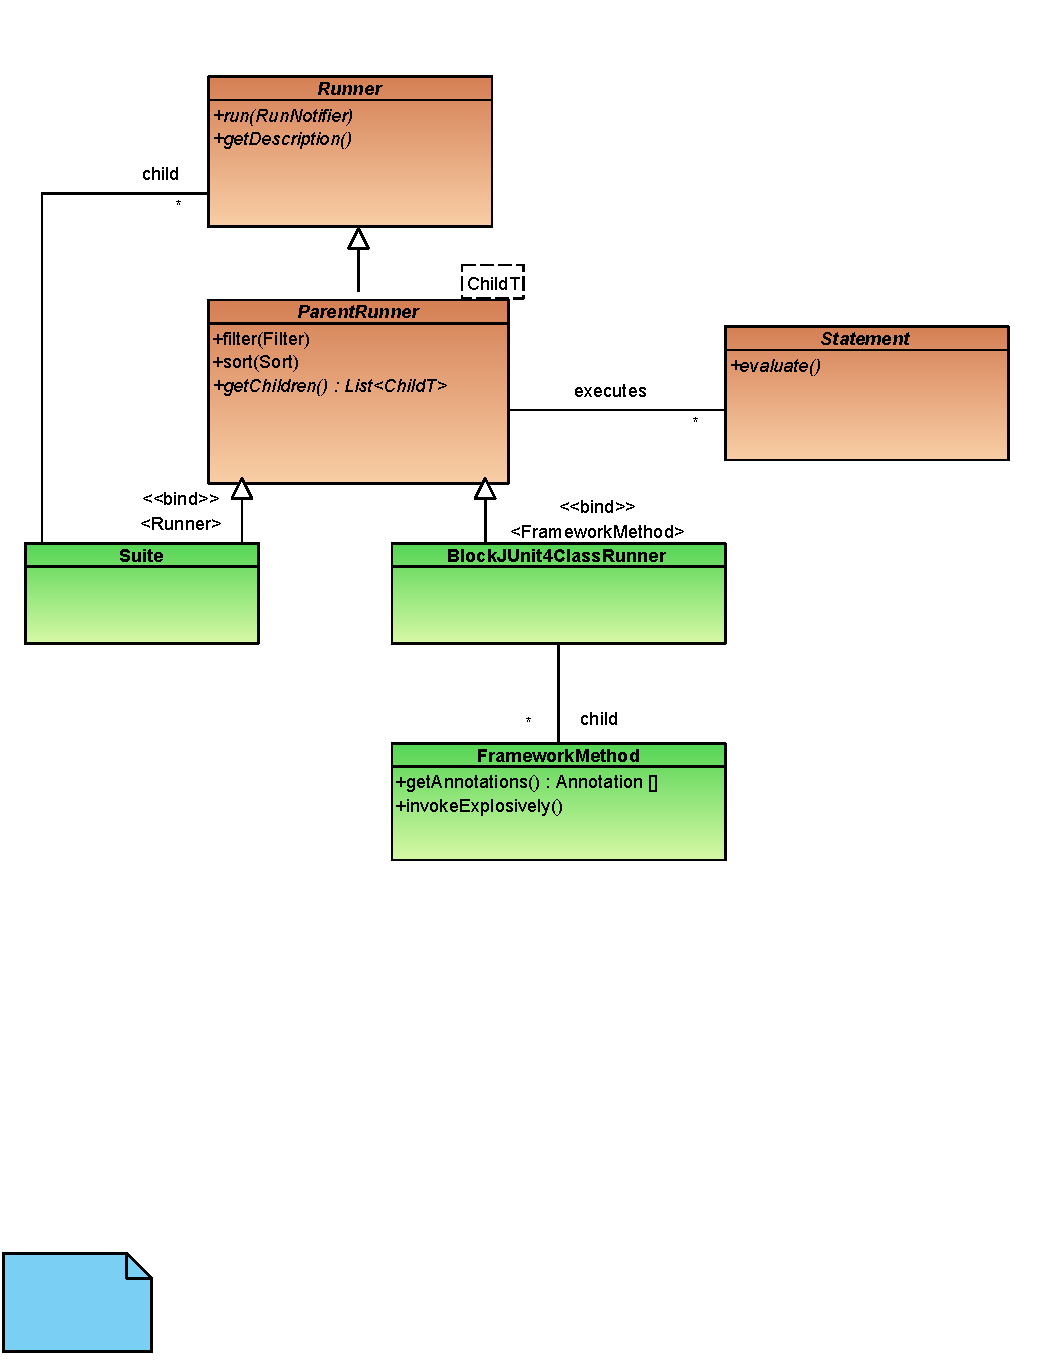
\includegraphics[width=0.65\textwidth]{ClassDiagramRunner}
	\caption{Klassendiagramma van de belangrijkste \emph{Runner}s.}
	\label{fig:diagrams:Runner}
\end{figure}

Er zijn twee belangrijke klassen die van de \emph{ParentRunner}-klasse overerven. Enerzijds is er de klasse \emph{org.junit.runners.Suite}, die een verzameling van \emph{Runner}s voorstelt en zo een hi\"erarchie in de uitvoer van testen toelaat. Anderzijds is er \emph{org.junit.runners.BlockJUnit4Runner}, die een \emph{Runner} voorstelt voor een enkele testklasse, met een verzameling van testmethodes als children. Dit is de \emph{Runner} die de eigenlijke testmethodes uitvoert.

Backwards compatibiliteit met versie v3.x wordt ondersteund door aangepaste \emph{Runner}s die een v3.x test wrappen.

\subsection{Aanmaken van Runners: Requests en Computers}

Het is mogelijk om een \emph{Runner} rechtstreeks aan te maken, maar in JUnit is het de bedoeling dat een \emph{Runner} gecre\"eerd wordt met behulp van de klasse \emph{org.junit.runner.Request}. Deze stelt een beschrijving voor van tests die uitgevoerd moeten worden, door middel van een \emph{Runner} die er aan kan opgevraagd worden. Een \emph{Request} kan aangemaakt worden vanuit een enkele klasse of een reeks klassen. Achter de schermen wordt er via een \emph{org.junit.interal.builders.AllDefaultPossibilitiesBuilder} een \emph{Runner} gecre\"eerd voor de opgegeven klasse of reeks van klassen.

In dit proces zit ook nog een \emph{org.junit.runner.Computer} verwerkt. Dit is een strategie voor het schedulen van \emph{Runner}s. Deze kunnen namelijk serieel gedraaid worden of parallel. Deze laatste functie is echter nog experimenteel.

\subsection{Uitvoeren van Runners: Statements en Rules}

Een \emph{org.junit.runners.model.Statement} stelt acties voor die genomen worden bij het aanroepen van zijn methode \emph{evaluate()}. Met meerdere \emph{Statement}s wordt het mogelijk om een uitvoering te regelen en te manipuleren. In een \emph{Statement} kan bijvoorbeeld met behulp van reflectie een methode-aanroep gedaan worden om een testmethode uit te voeren. Deze \emph{Statement}s kunnen gewrapped worden door andere \emph{Statement}s om zo hun gedrag uit te breiden of te veranderen.

Een flexibelere manier om het gedrag van een test te veranderen is het gebruik van \emph{org.junit.rules.TestRule}s. Deze hebben een methode \emph{apply(Statement, Description)} die een \emph{Statement} teruggeeft. Op deze manier kan het wijzigen of wrappen van \emph{Statement}s dus via overerving van een \emph{TestRule} gedaan worden. In JUnit wordt er een onderscheid gemaakt tussen een \emph{org.junit.Rule}, die gespecificeerd wordt als annotatie op velden en methodes, en een \emph{org.junit.ClassRule}, die gespecificeerd wordt als annotatie op klassen.

\emph{ParentRunner} is de belangrijkste \emph{Runner}-implementatie. Achter de schermen worden de childrunners, childtesten of andere children uitgevoerd door ze in een \emph{Statement} te plaatsen. Deze \emph{Statement} wordt echter niet rechtstreeks uitgevoerd, ze wordt eerst gewrapped door andere \emph{Statement}s. \emph{ParentRunner} gebruikt de volgende wrapper \emph{Statement}s:

\begin{description}
\item[RunBefores] voert methodes uit voor de uitvoer van de gewrapte \emph{Statement}. Deze worden gespecificeerd door een \emph{@Before}-annotatie die geplaatst wordt op een testmethode of testklasse.
\item[RunAfters] analoog, maar wordt uitgevoerd na de gewrapte statement en gespecificeerd door een \emph{@After}-annotatie.
\item[RunRules] voert \emph{TestRule}s uit op de \emph{Statement} om zo een gewijzigde \emph{Statement} te bekomen die het gedrag voorstelt van deze \emph{TestRule}s.
\end{description}

De \emph{BlockJUnit4ClassRunner}-klasse, die methodes als children heeft, voert zijn methodes ook uit in een \emph{Statement}. Hierin wordt voor elke testmethode een nieuwe instantie aangemaakt van de testklasse, om isolatie van de verschillende testmethodes te bekomen. Deze \emph{Statement} wordt opnieuw gewrapped, hier door de \emph{Statement}s:

\begin{description}
\item[ExpectException] werpt een fout op als de gewrapte \emph{Statement} niet de verwachte exception opwerpt, zodat de test faalt.
\item[FailOnTimeout] werpt een fout op als de gewrapte \emph{Statement} te lang doet over zijn uitvoer, zodat de test faalt.
\item[RunBefores, RunAfters en RunRules] werken hetzelfde als bij \emph{ParentRunner}.
\end{description}

De eerste vier zijn hierbij als deprecated gedeclareerd, zodat het eigenlijk aangeraden is om voor gewijzigde uitvoer altijd \emph{TestRule}s te gebruiken.

\subsection{}

\subsection{Standaard JUnit uitvoering}

De klasse die de main methode bevat in het JUnit project is \emph{JUnitCore}.
\emph{JUnitCore} is een facade voor het uitvoeren van testen.
In figuur \ref{fig:junitsequence} is het sequence diagram weergegeven.
\emph{JUnitCore} implementeert weinig functionaliteit.
Via de ``run()'' methoden wordt de uitvoering van de testen gestart.
Deze testen worden eigenlijk uitgevoerd in een \emph{Suite}.
De manier waarop deze \emph{Suite} verkregen wordt is niet eenvoudig.
\emph{JUnitCore} maakt een statische oproep naar \emph{Request},
\emph{Request} maakt dan een \emph{Computer} en een
\emph{AllDefaultPossibilitiesBuilder}, daarna maakt de \emph{Computer}
een \emph{Suite} aan.
Deze \emph{Suite} maakt gebruikt van de \emph{AllDefaultPossibilitiesBuilder}
om een \emph{RunnerBuilder} te verkrijgen (dit is niet in het diagram
ge\"expliciteerd), de \emph{AllDefaultPossibilitiesBuilder} vult deze in met
bvb. een \emph{IgnoreBuilder} die ervoor zorgt dat een test niet uitgevoerd
wordt.
De statische oproep in \emph{Request} cre\"eert dan een \emph{Request}-object
dat de aangemaakte \emph{Suite} als runner bevat.
Om de tests daadwerkelijk te starten vraagt \emph{JUnitCore} de runner op
van de \emph{Request} en start deze met ``run()''.





\section{Evaluatie van het ontwerp}

%Een evaluatie van het ontwerp. Wat zijn sterke en zwakke punten van het ontwerp. Bespreek
%ook het gebruik (of het niet-gebruik) van patronen. Geef opnieuw sterke en zwakke punten
%van het ontwerp op dit vlak.

\subsection{Sterke en zwakke punten}

\subsection{Gebruik van patronen}

Er worden verschillende software design patterns gebruikt in JUnit. 
Hieronder volgt een overzicht van een aantal design patterns en voorbeelden van waar ze gebruikt worden.

\subsubsection{Factory Method}
In de klasse \emph{runners.model.RunnerBuilder} bevindt zich een Factory Method om \emph{runner.Runner}s aan te maken, namelijk \emph{runnerForClass()}. 
In de documentatie wordt ook aangegeven dat de methode in een subklasse ge\"implementeerd moet worden om de juiste \emph{Runner} terug te geven.

\subsubsection{Observer}
De structuur \emph{runner.Runner}-\emph{runner.RunNotifier}-\emph{runner.RunListener} kan gezien worden als een vorm van Observer structuur. 
De klasse \emph{Runner} wordt ge\"instanti\"eerd met een \emph{RunNotifier}, die notificatiemethoden bevat die aangeroepen worden door de klasse \emph{Runner}. 
Aan een \emph{RunNotifier} object kan dan een \emph{RunListener} worden toegevoegd (via de \emph{Runner}, de \emph{addListener()} methode van \emph{RunNotifier} is wel public, maar de documentatie geeft aan dat deze enkel voor intern gebruik is en dat de listener moet worden toegevoegd door de \emph{Runner}). 
Dit maakt het mogelijk om tijdens het uitvoeren van een testrun op verschillende manieren te reageren op gebeurtenissen die kunnen voorkomen tijdens het uitvoeren van testen (zoals wanneer een test begint of eindigt, een Exception opgegooid wordt, ...).

\subsubsection{Composite}
Het Composite pattern wordt gebruikt in een aantal structuren. Een eerste voorbeeld hiervan is de interface \emph{rules.TestRule}, verschillende implementerende Leaf-klassen en de Composite \emph{rules.RuleChain}. 
\emph{RuleChain} implementeert \emph{TestRule} en bevat zelf kinderen die ook \emph{TestRule} objecten zijn.
\\
Ook de structuur \emph{runner.Runner} - \emph{internal.runners.ErrorReportingRunner},\ldots - \emph{runners.ParentRunner} is een voorbeeld van een Composite pattern. 
Een \emph{ParentRunner} kan verschillende kinderen bevatten die ook \emph{Runner}s zijn. 
Op deze manier kan het gedrag van de \emph{Runner} tijdens het uitvoeren van testen aangepast worden (bijvoorbeeld om slim om te gaan met opgegooide Exceptions).
\\
De ontwerpers van JUnit zelf vermelden dat de klasse \emph{runner.Description} niet als Composite ge\"implementeerd is omdat er geen logica in uitgevoerd wordt. Ze bevat enkel informatie.

\subsubsection{Command}
Het Command pattern is terug te vinden in veel van de klassen van de package rules. 
Een goed voorbeeld hiervan is \emph{rules.ExternalResource}, die toestaat om voor een test een externe bron in te laden. 
Deze functionaliteit is afgezonderd in de \emph{ExternalResource} klasse samen met methoden om voor en na het inladen iets te doen, een vorm van omkadering die typisch is voor het Command pattern. 

\subsubsection{Strategy}
De ontwerpers vermelden zelf in de documentatie van de klasse \emph{runner.Computer} dat deze bedoeld is als Strategy maar het is niet erg duidelijk aangezien er (buiten de klasse \emph{experimental.ParallelComputer}) maar \'e\'en klasse Computer is en er dus maar \'e\'en Strategy is.
\\
Iets gelijkaardig is er voor \emph{runners.model.RunnerScheduler}. Hier wordt ook expliciet vermeld dat het bedoeld is als Strategy. De enige plaatsen waar gebruik gemaakt wordt van het pattern is echter in enkele methoden die anonieme inwendige klassen defini\"eren.


\subsubsection{Visitor}
Dit pattern is niet echt op een zuivere manier toegepast, maar het kan herkend worden in de klassen \emph{runner.manipulation.Filter} en \emph{runner.manipulation.Filterable}. 
In dit geval is de \emph{Filter} de Visitor die uitbreidingen van de klasse \emph{runner.Description} bezoekt. 
Er worden dan \emph{Description}s gefilterd van testen die niet uitgevoerd moeten worden. 
\\
Sortable is een analoge vorm van pseudo-Visitor die kan toegepast worden op een \emph{Description}-hi\"erarchie.
\\
Het gaat hier niet om een echte instantie van het Visitor pattern omdat er in \emph{Filter} geen onderscheid gemaakt wordt tussen verschillende soorten \emph{Filterable} objecten maar alleen of ze \emph{Filterable} zijn of niet.



%%%%%%%%%%%%%%%%%%%%%%%%%%%%%%%%%%%%%%%%%%%%%%%%%%%%%%%%%%%%%%%%
%
%		Beschrijving en evaluatie van de analyse tools
%
%%%%%%%%%%%%%%%%%%%%%%%%%%%%%%%%%%%%%%%%%%%%%%%%%%%%%%%%%%%%%

\section{Beschrijving en evaluatie van de analyse tools}

Voor de analyse van JUnit werden er vier analyse tools gebruikt namelijk: \emph{X-Ray} \cite{X-Ray}, \emph{AgileJ Structureviews} \cite{AgileJ Structureviews} , \emph{Design Pattern Detection Tool} \cite{Design Pattern Detection Tool} en \emph{InFusion} \cite{Infusion}. Om \emph{X-Ray} beter de begrijpen werd er ook nog gekeken naar \emph{CodeCity} \cite{CodeCity}.


\subsection{X-Ray} 
\emph{X-Ray} is een visualisatie tool die de complexiteit van de klassen weergeeft. Figuur \ref{fig:X-Ray} geeft dit weer. De rechthoeken geven de klassen weer. De breedte van een rechthoek geeft het aantal methodes weer en de lengte het aantal lijnen code. Overerving wordt weergegeven via een boomstructuur. Met \emph{X-Ray} kan je ook opzoeken wie de parents zijn van een klasse of de children. Via kleuren geven ze ook het type klasse mee: Abstract, Concrete, Interface en Internal Classes. Door een klasse te selecteren kan men de dependencies zien van deze klasse via rode lijnen die deze klasse verbinden met de afhankelijke klassen. Het nadeel aan \emph{X-Ray} is dat de klassen zeer uitgespreid in de breedte worden weergegeven. \\
\emph{CodeCity} geeft een goed beeld maar er is weinig flexibiliteit. Er kunnen packages verborgen worden maar dan is er een witruimte op de plaats van de package. Het werd vooral gebruikt om een overview te krijgen van het project. Via \emph{CodeCity} kon er ook gekeken worden naar de dependencies. 
%TODO Foto van codeCity


\begin{figure}[hb!]
	\centering
	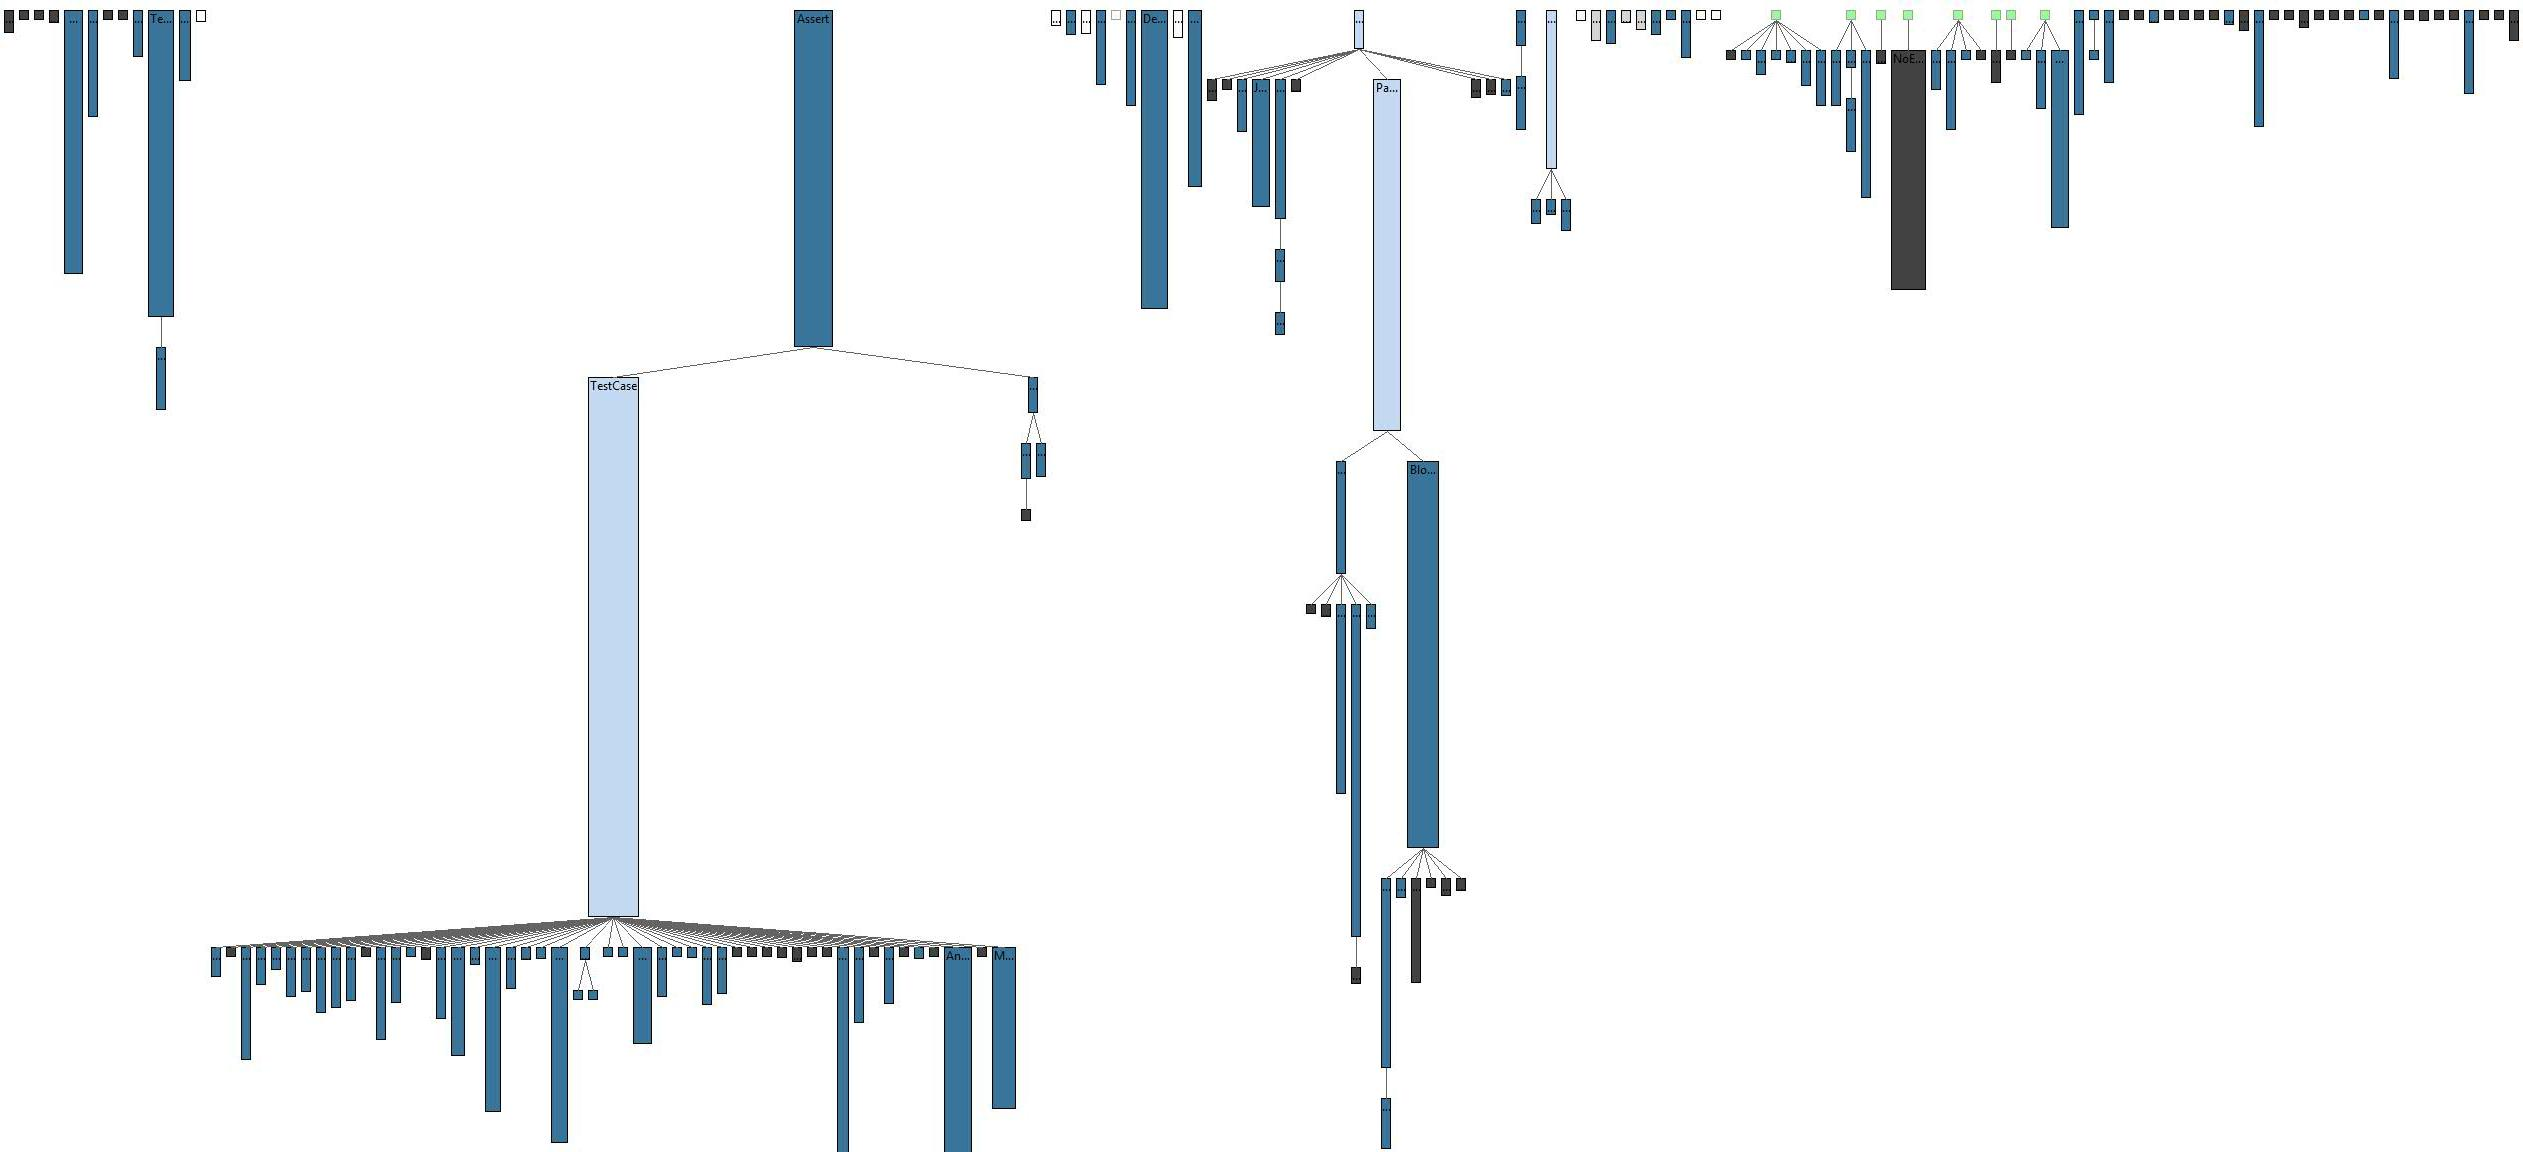
\includegraphics[width=0.70\textwidth]{XRayComplexity}
	\caption{X-Ray: polymetric view}
	\label{fig:X-Ray}
\end{figure}

\subsection{AgileJ Structureviews}
\emph{AgileJ Structureviews} is een tool die klassendiagramma's kan genereren. Figuur \label{fig:AgileJklassendia} geeft een voorbeeld weer van een klassendiagramma dat gegenereerd is via \emph{AgileJ}.\\
Onze klassendiagramma's zijn gebaseerd op de klassendiagramma's die we via \emph{AgileJ} gegenereerd hebben. De klassendiagramma's die gegenereerd werden via \emph{AgileJ} bevatte alle methodes en velden waardoor er geen duidelijk overzicht was. Via filters konden deze methoden gefilterd worden. Een pluspunt aan het programma was dat het onderscheid tussen abstracte of concrete klassen bepaald kon worden door het gebruik van filters. Voor dit onderscheid werd er gebruik gemaakt van verschillende kleuren.\\



\begin{figure}[h!]
	\centering
	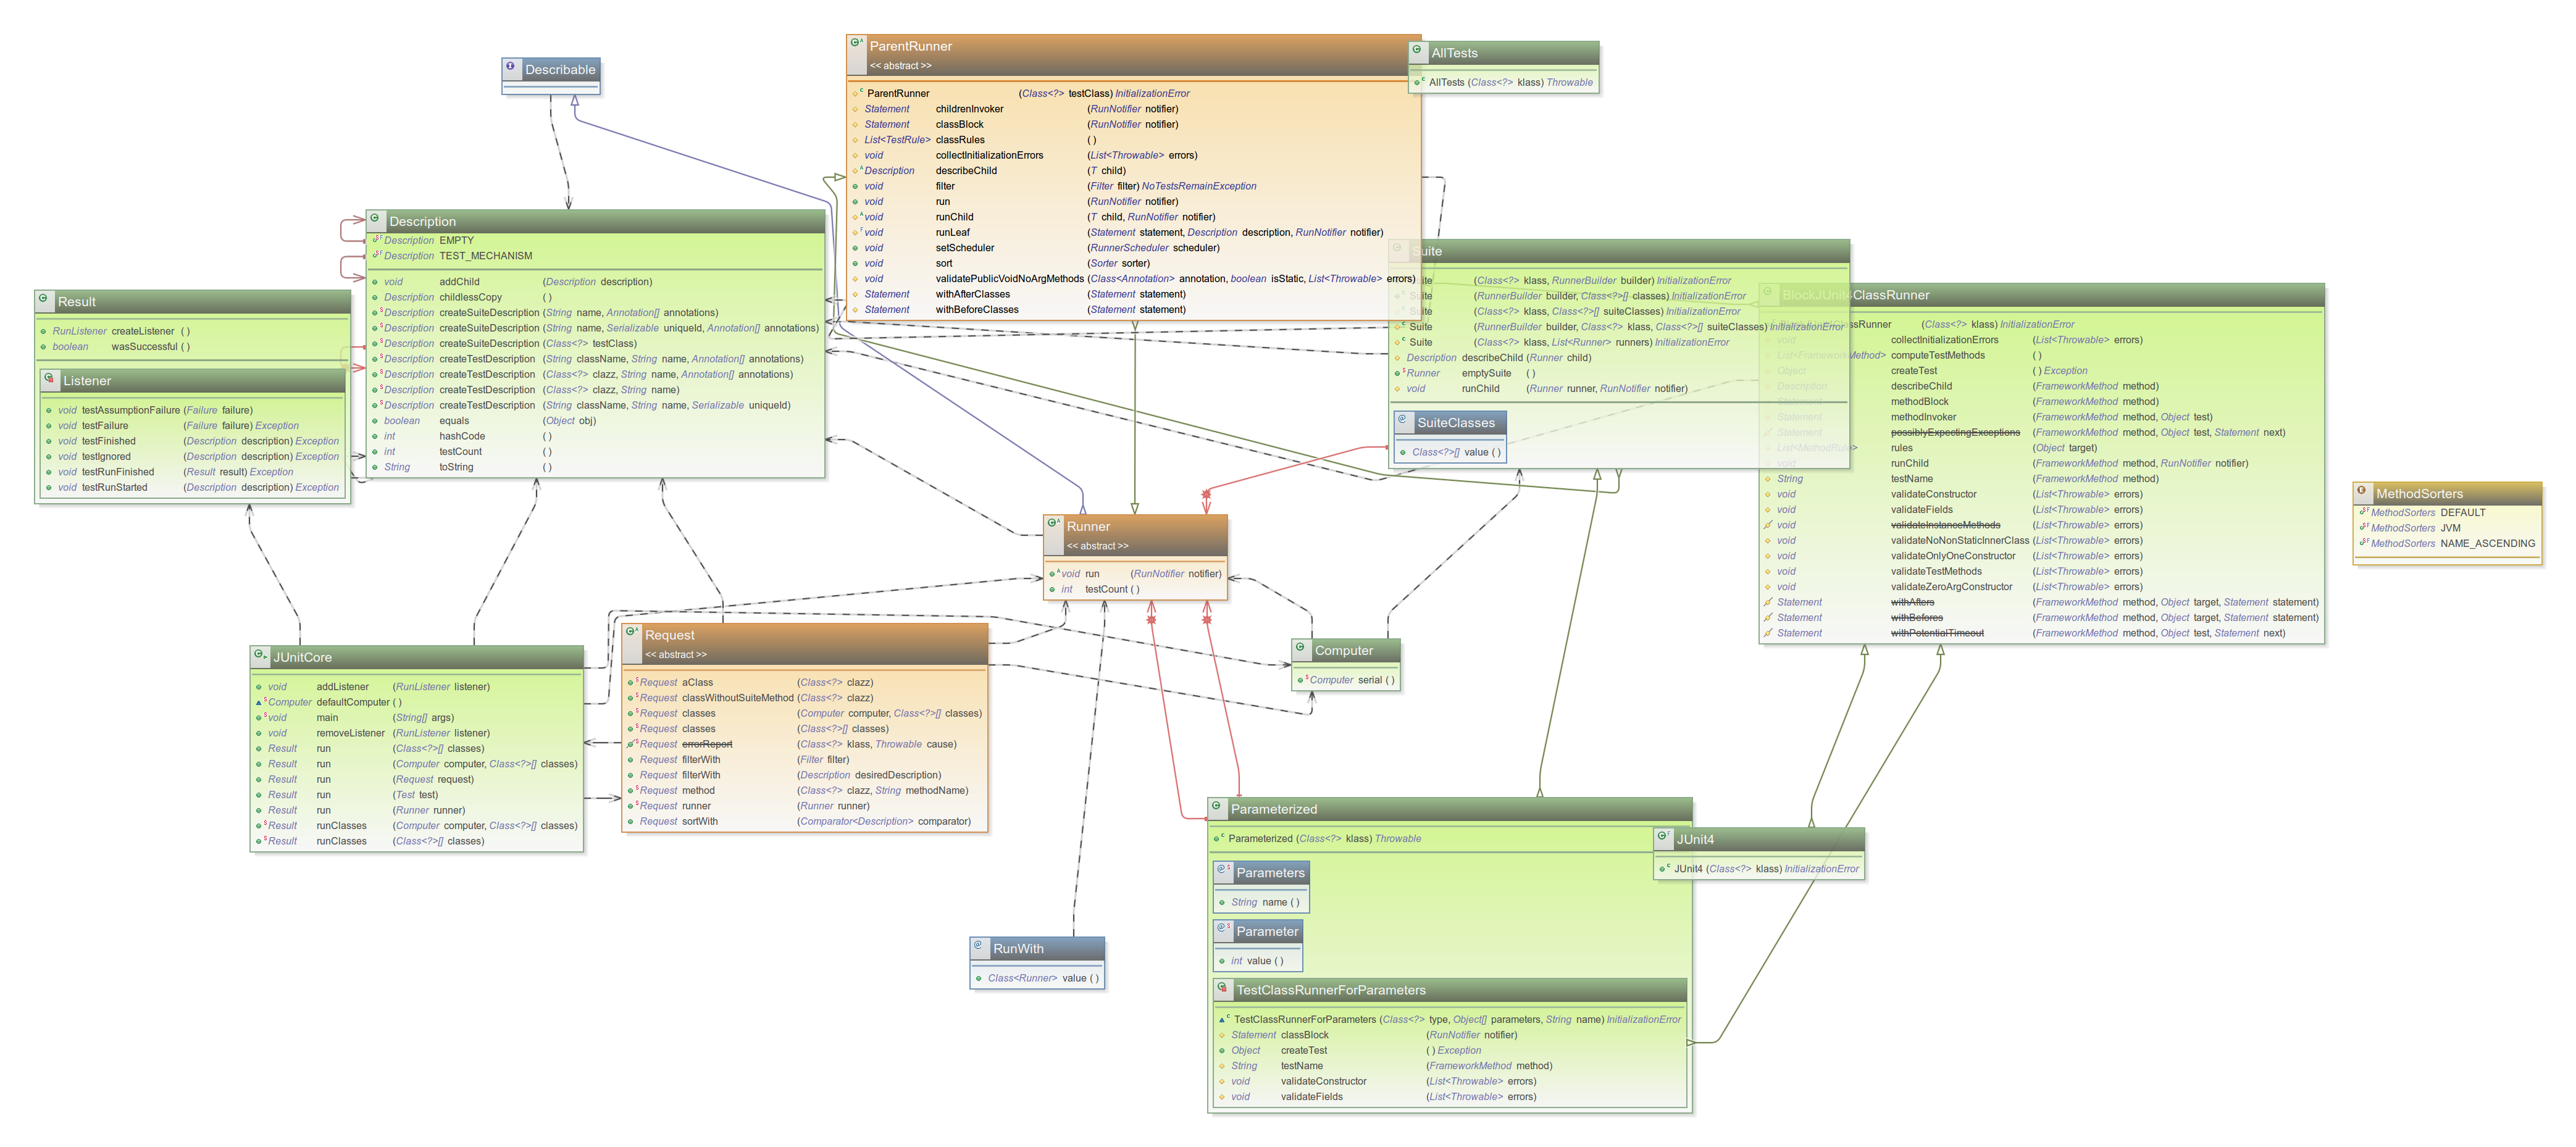
\includegraphics[width=0.65\textwidth]{AgileJKlassendiagramma}
	\caption{AgileJ Sturcutureviews: klassendiagramma}
	\label{fig:AgileJKlassendia}
\end{figure}

\subsection{Design Pattern Detection Tool}
\emph{Design Pattern Detection Tool} is een tool die het programma gaat checken op bepaalde patterns. Een overzicht van de patterns die gevonden zijn via de tool is te zien op de figuur \ref{fig:DesignPatterns}. Deze tool werkt op de gecompileerde code. Het maakt een graph aan van de verschillende klassen en gebruikt graph matching om de patterns te herkennen.  Dit geeft gemengde resultaten. Sommige van de herkende patterns zijn correct, andere lijken oppervlakkig op het gewenste pattern maar komen er bij nader inzien niet mee overeen. 
Deze tool is vooral een goede leidraad om patterns te beginnen zoeken in JUnit.\\

\begin{figure}[h!]
	\centering
	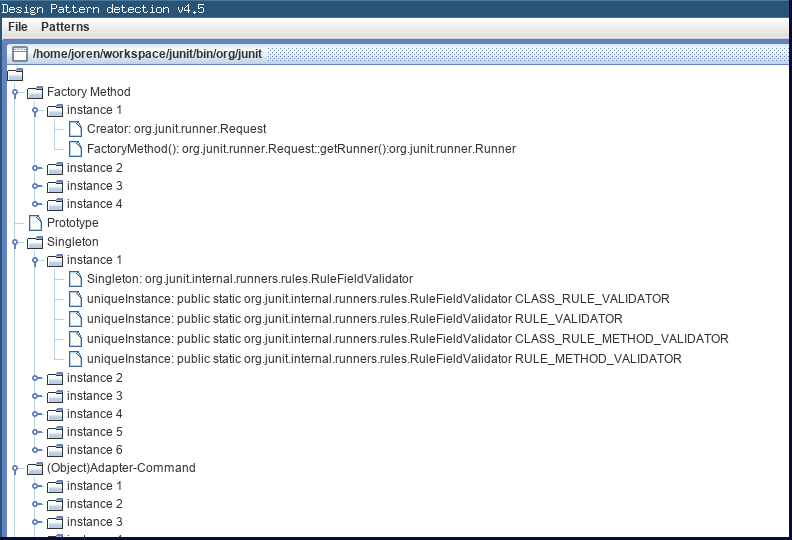
\includegraphics[width=0.65\textwidth]{Patterns1}
	\caption{Overzicht van de patterns}
	\label{fig:DesignPatterns}
\end{figure}

\subsection{InFusion}
\emph{InFusion} berekent een groot aantal metrics die niet allemaal even verstaanbaar zijn. Dit wordt samengevat in een overview piramid. InFusion berekent ook allerlei scores die vermoedelijke code smells identificeren. Het bied ook een polymetric view aan waarin verschillende perspectieven genomen kunnen worden zoals coupling, complexity en encapsulation. De kleuren van de polymetric view passen zich aan aan de verschillende perspectieven. Een voorbeeld screenshot van InFusion wordt weergegeven in figuur~\ref{fig:InFusion}.


\begin{figure}[h!]
\centering
	\begin{subfigure}[h]{0.65\textwidth}
		\centering
		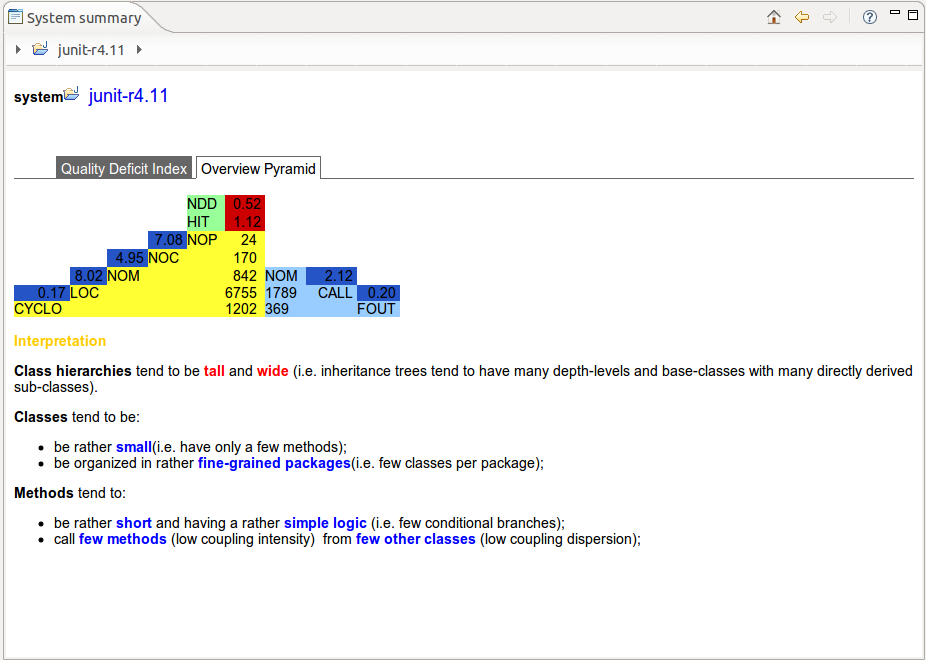
\includegraphics[width=\textwidth]{inFusion1}
		\caption{Overview Pyramid}
	\end{subfigure}
	\begin{subfigure}[h]{0.65\textwidth}
		\centering
		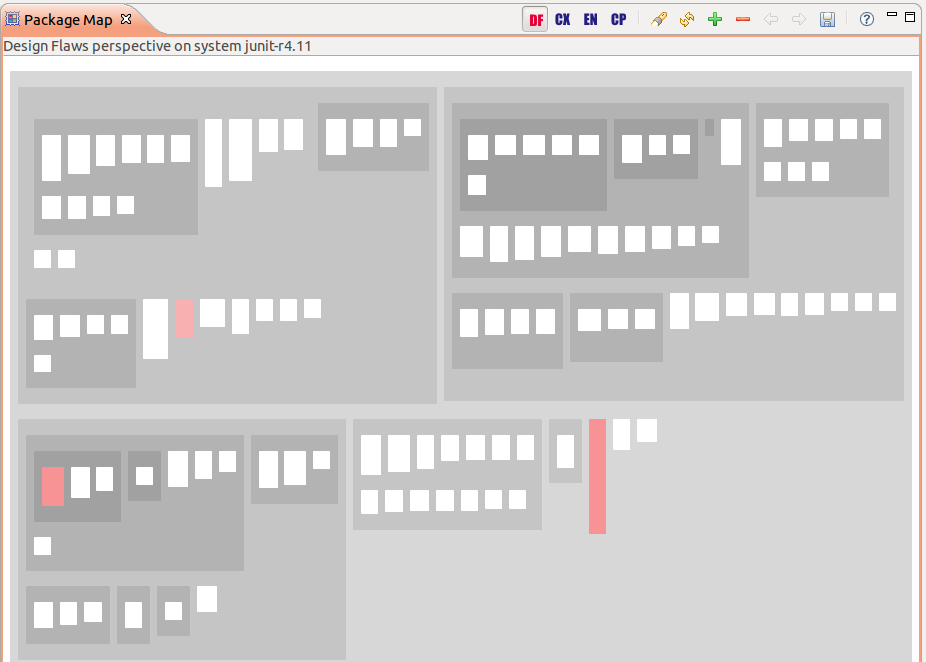
\includegraphics[width=\textwidth]{inFusion2}
		\caption{Design flaw perspective}
	\end{subfigure}
\caption{Screenshots van InFusion}
\label{fig:InFusion}
\end{figure}



\section{Evaluatie testen}

\section{Samenvatting}

\section{Projectbeheer}

Het was in het begin niet altijd even makkelijk om visualisatietools te vinden die we ook daadwerkelijk werkend kregen.
Wij zijn vrij laat begonnen aan het project omdat onze groep nog niet samengesteld was in het begin van de eerste week. In de eerste week zijn we bijeengekomen om samen de opdracht te lezen en de verschillende visualisatie tools op te zoeken en onder elkaar te verdelen. 

Er werd steeds in een tabel bijgehouden wie wanneer aan wat had gewerkt. Dit gaf eveneens een zicht op wat er al klaar was en wat nog moest gebeuren. \\
Tabel~\ref{tab:werkuren} geeft weer hoeveel tijd in het project gestoken werd per persoon per onderdeel. Figuur~\ref{fig:werkverdeling} toont wie aan welke aspecten van het project heeft gewerkt.

%TODO laatste week aanvullen!!
\begin{table}[h]
\begin{center}
    \begin{tabular}{ r | c  c  c  c  c  c}
     & Joren & Toon & Stef & Sophie \\ \hline
    Algemeen & 9u00 & 9u00 & 8u55 & 7u15\\
   	Tools & 10u00 & 22u10 & 12u00 & 9u00 \\
	Analyse & 14u00 & 25u05 & 9u00 & 8u00 \\
	Ontwerp & 00u00 & 00u00 & 00u00 & 00u00 \\
	Implementeren & 00u00 & 00u00 & 00u00 & 00u00\\
	Verslag & 11u30 & 7u00 & 17u10 & 15u00 \\
	Totaal & & & & 
    \end{tabular}
    \caption{Overzicht werkuren per onderdeel}
    \label{tab:werkuren}
\end{center}
\end{table}

%TODO figuren updaten
\begin{figure}[h!]
        \centering
        \begin{subfigure}[hb]{0.15\textwidth}
                \centering
                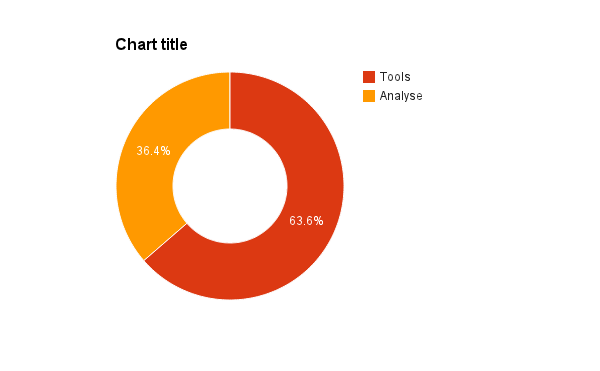
\includegraphics[width=\textwidth]{chart_2}
                \caption{Joren}
        \end{subfigure}%
        \begin{subfigure}[hb]{0.15\textwidth}
                \centering
                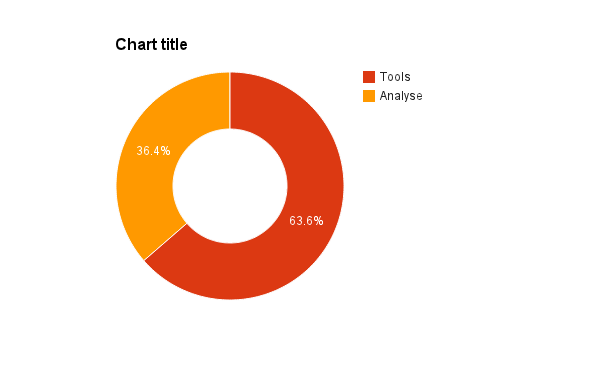
\includegraphics[width=\textwidth]{chart_3}
                \caption{Toon}
        \end{subfigure}%
        \begin{subfigure}[hb]{0.15\textwidth}
                \centering
                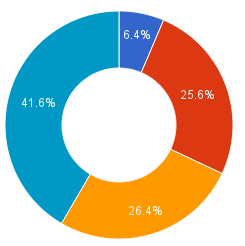
\includegraphics[width=\textwidth]{chart_4}
                \caption{Stef}
        \end{subfigure}%
        \begin{subfigure}[hb]{0.15\textwidth}
                \centering
                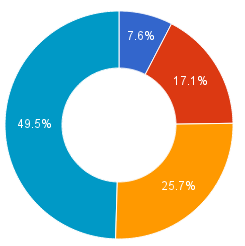
\includegraphics[width=\textwidth]{chart_5}
                \caption{Sophie}
        \end{subfigure}%
                \begin{subfigure}[hb]{0.15\textwidth}
                \centering
                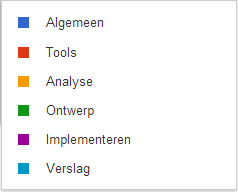
\includegraphics[width=\textwidth]{legende}
                \caption{Legende}
        \end{subfigure}%


 \caption{Weergave van de werkverdeling}
\label{fig:werkverdeling}
\end{figure}

\newpage
\begin{flushleft}
\begin{thebibliography}{4}

\bibitem{X-Ray}
\emph{X-Ray}
\begin{scriptsize}
geraadpleegd op 11/10/2013 via: \mbox{http://xray.inf.usi.ch/xray.php} en \mbox{https://marketplace.eclipse.org/content/x-ray-software-visualization}
\end{scriptsize}

\bibitem{AgileJ Structureviews}
\emph{AgileJ Structureviews}
\begin{scriptsize}
geraadpleegd op 11/10/2013 via: \mbox{http://www.agilej.com/}
\end{scriptsize}

\bibitem{Design Pattern Detection Tool}
\emph{Design Pattern Detection Tool}
\begin{scriptsize}
geraadpleegd op 15/10/2013 via: \mbox{http://java.uom.gr/~nikos/pattern-detection.html} versie  Design Pattern detection Tool (version 4.5 - build 28/05/2010)
\end{scriptsize}

\bibitem{inFusion}
\emph{InFusion Hydrogen}
\begin{scriptsize}
geraadpleegd op 17/10/2013 via: \mbox{http://www.intooitus.com/products/infusion/download} versie InFusion Hydrogen v1.8.0
\end{scriptsize}

\bibitem{CodeCity}
\emph{CodeCity}
\begin{scriptsize}
geraadpleegd op 9/10/2013 via: \mbox{http://www.inf.usi.ch/phd/wettel/codecity.html} 
\end{scriptsize}

\end{thebibliography}
\end{flushleft}

\end{document}



